\documentclass[journal,12pt,two column]{IEEEtran}
\usepackage[utf8]{inputenc}
\usepackage{amsmath}
\usepackage[margin = 0.8in]{geometry}
\usepackage{float}
\usepackage{graphicx}
\graphicspath{{images/}}
\setlength{\columnsep}{1.4cm}


\title{AI1110 Assignment 1}
\author{Tejal Kulkarni CS21BTECH11058}
\date{March 2022}

\begin{document}
\maketitle
\textbf{Q8(c):} The printed price of an air conditioner is  Rs.45,000/-. The wholesaler allows a discount of 10\% to the shopkeeper. The shopkeeper sells the article to the customer at a discount of 5\% of the marked price. Sales tax (under VAT) is charged at the rate of 12\% at every stage. Find:
\begin{enumerate}
\item[(i)]VAT paid by the shopkeeper to the government.
\item[(ii)]The total amount paid by the customer inclusive of tax. 
\end{enumerate}
\textbf{Solution:}
\begin{table}[ht!]
\caption{\textbf{Table with input and output variables, their symbols, their formulae and values:}}
    \label{table:1}
   \begin{tabular}{|p{3.5cm}|c|c|c|}
       \hline
     \textbf{Description}  & \textbf{Symbol} &  \textbf{Formula}  &  \textbf{Value} \\
       \hline
       \hline
       Marked Price & MP & - & Rs.45000 \\  
       \hline
       Discount for shopkeeper & d1 & - & 10\% \\
       \hline
       Discount amount for shopkeeper & disc1 & $\text{MP}\times\dfrac{d1}{100}$ & Rs.4500\\
       \hline
       Selling Price for shopkeeper & SP1 & $\text{MP} -  \text{disc1}$ & Rs.40500 \\
       \hline
       Sales Tax & s & - & 12\% \\
       \hline
       Tax amount for shopkeeper & t1 & $\text{SP1}\times\dfrac{s}{100}$ & Rs.4860\\
       \hline
       Discount for customer & d2 & - & 5\% \\
       \hline
       Discount amount for customer & disc2 & $\text{MP}\times\dfrac{d2}{100}$ & Rs.2250 \\
       \hline
       Selling Price for customer & SP2 & $\text{MP} - \text{disc2}$ & Rs.42750 \\
       \hline
       Tax amount for customer & t2 & $\text{SP2}\times\dfrac{s}{100}$ & Rs.5130\\
       \hline
       VAT paid by shopkeeper to govt. & V & $\text{t2} - \text{t1}$ & ?\\
       \hline
       Total Amount paid by customer & T & $\text{SP2} + \text{t2}$ & ?\\
       \hline
       
    \end{tabular}

\end{table}

Formulae used according to the Table \ref{table:1}:\\
\begin{align}
  \text{disc} &= \text{MP}\times\frac{\text{d}}{100}\hspace{1cm}...\\ 
  \text{SP} &= \text{MP} - \text{disc} \hspace{1cm}...\\ 
  \text{t} &= \text{SP}\times\frac{\text{s}}{100}\hspace{1cm}...
\end{align}
Marked  Price(MP) = Rs.45,000/- \\
Sales  Tax(s) = 12\% \\
Discount  for  shopkeeper (d1) = 10\% \\ \\
Discount  amount for shopkeeper (disc1)   \begin{equation*}
    = 45000\times\frac{10}{100} = Rs.4500 \hspace{1cm}... by \hspace{0.2cm} (1) 
    \end{equation*} 
Selling Price for shopkeeper (SP1) = \begin{equation*}
    45000 - 4500 = Rs.40500 \hspace{1cm}... by \hspace{0.2cm} (2)
\end{equation*}
Sales Tax for shopkeeper(t1)  \begin{equation*} 
    = 40500\times\frac{12}{100} =  Rs.4860 \hspace{1cm}... by \hspace{0.2cm} (3)
\end{equation*}
Discount for customer (d2) = 5\% \\ \\
Discount amount for customer(disc2)  
\begin{equation*} 
    =  45000\times\frac{5}{100} = Rs.2250 \hspace{1cm}... by \hspace{0.2cm} (1)
    \end{equation*}
Selling Price for customer (SP2)  \begin{equation*}
   = 45000 - 2250 =  Rs.42750 \hspace{1cm}... by \hspace{0.2cm} (2) 
\end{equation*}
Sales tax for customer (t2)  \begin{equation*}
   = 42750\times\frac{12}{100} = Rs.5130 \hspace{1cm}... by \hspace{0.2cm} (3)
\end{equation*} 
Hence,
\begin{enumerate}
\item[(i)]Tax for customer - Tax for shopkeeper = 
    VAT paid by shopkeeper to government(V)  
     \begin{equation*}
        = 5130 - 4860 = \fbox{Rs.270}
     \end{equation*}
\item[(ii)]Selling price for customer + Tax for customer = Total amount paid by customer(T) 
    \begin{equation*}
       = 42750 + 5130 = \fbox{Rs.47880}
   \end{equation*} 
\end{enumerate}

\begin{figure}[ht!]
     \centering
     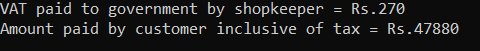
\includegraphics[scale = 1]{codeoutput2.png}
     \caption{The output of the program used for verification:}
     \label{fig:Figure 1}
\end{figure}

\end{document}
